\begin{figure}
    \centering
    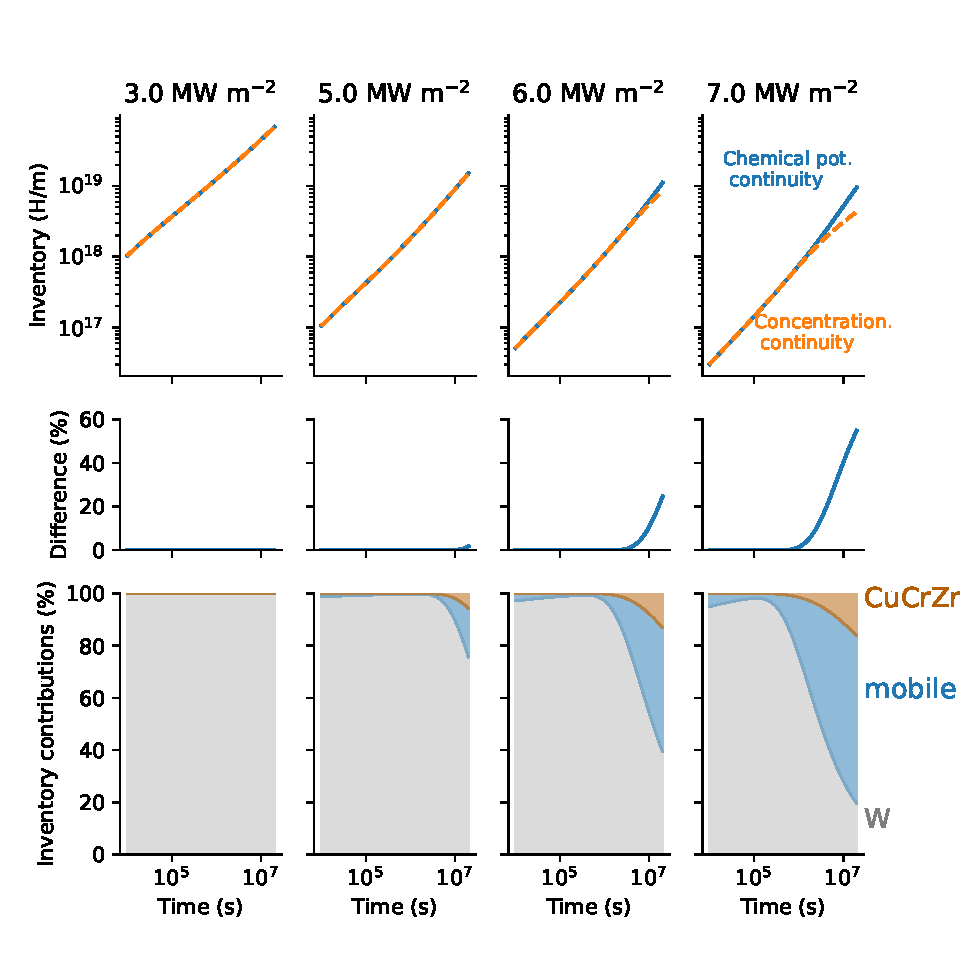
\includegraphics[width=\linewidth]{Figures/Chapter3/monoblocks/interface_condition/difference_w_wo_chemical_pot.pdf}
    \caption{Influence of chemical potential conservation on hydrogen inventory.}
    \labfig{influence of chemical potential on monoblock inventory}
\end{figure}


\begin{figure}
    \centering
    \begin{subfigure}{0.5\linewidth}
        \centering
        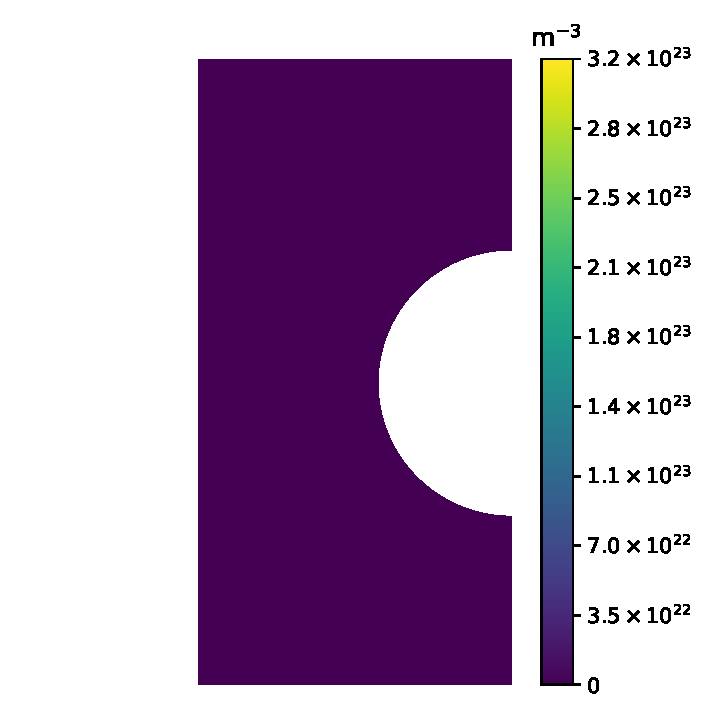
\includegraphics[width=\linewidth]{Figures/Chapter3/monoblocks/interface_condition/iter case/mobile_concentration.pdf}
        \caption{$c_\mathrm{m}$ (continuity of $c_\mathrm{m}$)}
    \end{subfigure}%
    \begin{subfigure}{0.5\linewidth}
        \centering
        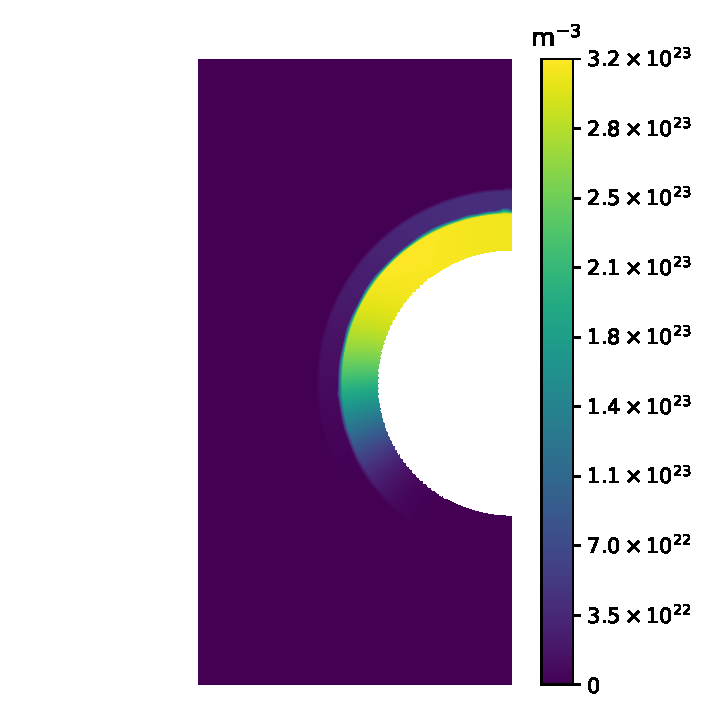
\includegraphics[width=\linewidth]{Figures/Chapter3/monoblocks/interface_condition/iter case/mobile_chemical_pot.pdf}
        \caption{$c_\mathrm{m}$ (continuity of chemical potential)}
    \end{subfigure}
    \begin{subfigure}{0.5\linewidth}
        \centering
        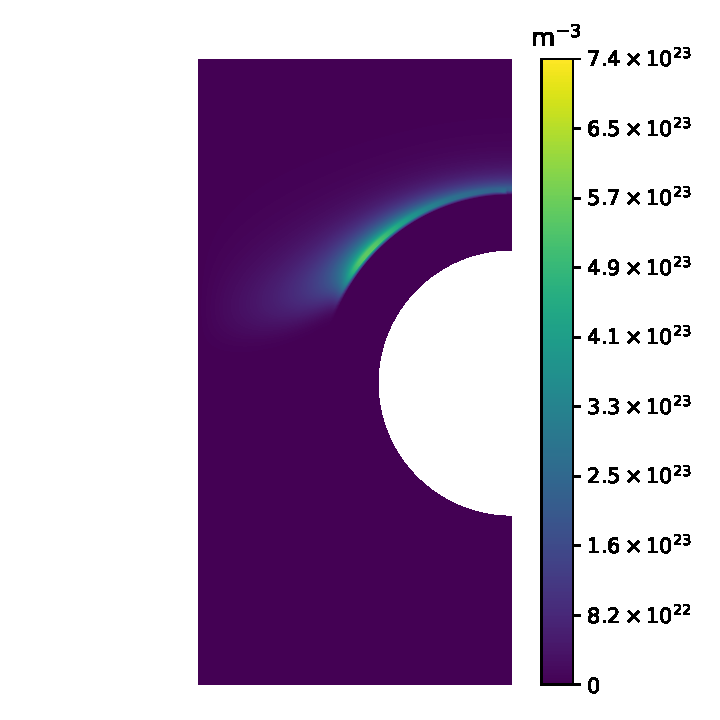
\includegraphics[width=\linewidth]{Figures/Chapter3/monoblocks/interface_condition/iter case/retention_concentration.pdf}
        \caption{Retention (continuity of $c_\mathrm{m}$)}
    \end{subfigure}%
    \begin{subfigure}{0.5\linewidth}
        \centering
        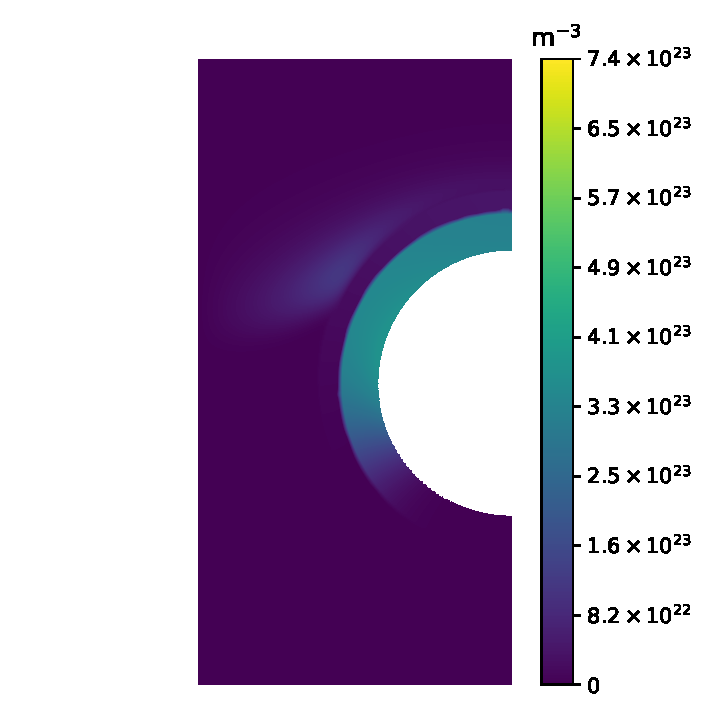
\includegraphics[width=\linewidth]{Figures/Chapter3/monoblocks/interface_condition/iter case/retention_chemical_pot.pdf}
        \caption{Retention (continuity of chemical potential)}
    \end{subfigure}
    \caption{Concentration fields at $t=\SI{2e7}{s}$}
    \labfig{concentration fields w/wo chemical potential}
\end{figure}

As monoblocks are made of several materials (tungsten, copper and CuCrZr), the continuity of chemical potential accross interfaces results in a mobile concentration jump (see \refsec{conservation of chemical potential}).
However, the problem could be simplified if, instead of ensuring the continuity of chemical potential, one ensured the continuity of mobile concentration across interfaces.
Indeed, this would allow to get rid of one equation and therefore reduce the computational time.
But is this simplification valid?

To verify its validity, 2D monoblock simulations are performed with chemical potential continuity (Equation \ref{eq: c/s conservation}) or mobile concentration continuity and the temporal evolution of the inventory was computed.
The implanted flux $\varphi_\mathrm{imp}$ was fixed to \SI{1.0e21}{m^{-2}.s^{-1}} and the heat flux $\varphi_\mathrm{heat}$ varied from \SI{3.0}{MW} to \SI{7.0}{MW}.

For the low flux cases (\SI{3}{MW} and \SI{5}{MW}), no difference was found (see \reffig{influence of chemical potential on monoblock inventory}).
For the case at \SI{6}{MW}, differences start to appear after \SI{3e6}{s} (\SI{7e5}{s} at \SI{7}{MW}).
After \SI{2e7}{s} of continuous exposure, the absolute difference at \SI{6}{MW} was 25 \% and 55 \% at \SI{7}{MW}.

This time of appearance of differences is identical to the time required for the hydrogen to migrate up to the W/Cu interface.
This is explained by the high solubility ratio between W, Cu and CuCrZr leading to a higher concentration of mobile particles in CuCrZr (see \reffig{concentration fields w/wo chemical potential}) and therefore a higher trapping rate.
Since the trap density in Cu is low, the global inventory is not affected by it.


\begin{figure}
    \centering
    \begin{subfigure}{0.5\linewidth}
        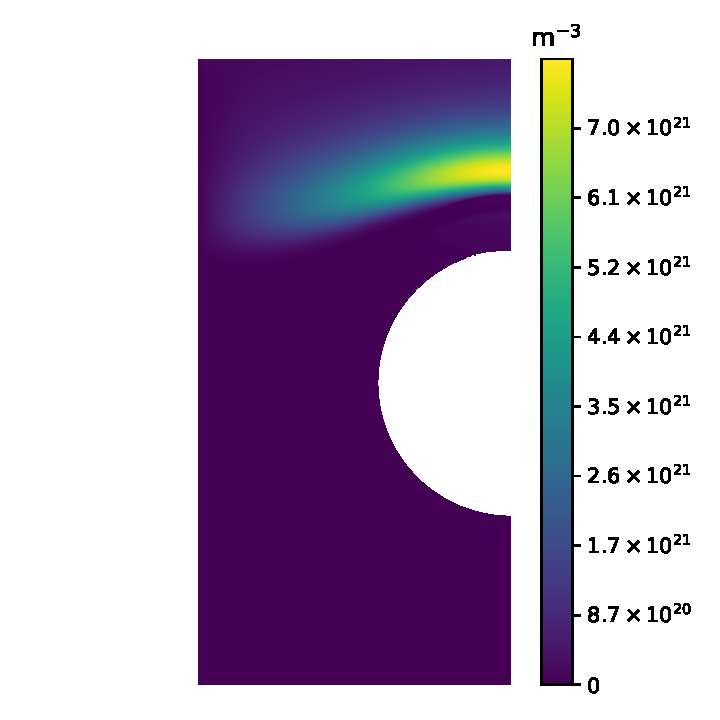
\includegraphics[width=\linewidth]{Figures/Chapter3/monoblocks/interface_condition/retention_chemical_pot_short_exposure.pdf}
        \caption{continuity of chemical potential}
    \end{subfigure}%
    \begin{subfigure}{0.5\linewidth}
        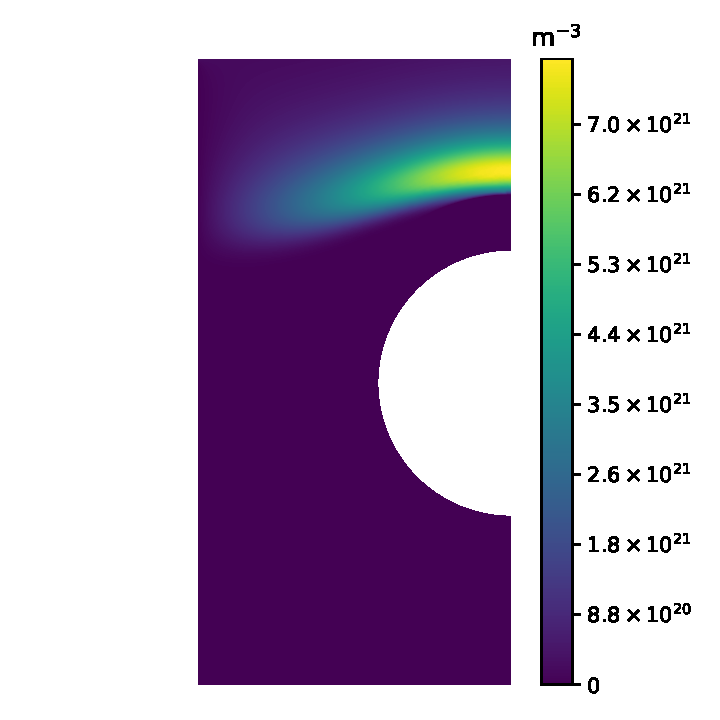
\includegraphics[width=\linewidth]{Figures/Chapter3/monoblocks/interface_condition/retention_concentration_short_exposure.pdf}
        \caption{continuity of mobile concentration}
    \end{subfigure}
    \caption{Retention fields at $t=\SI{6.1e4}{s}$.}
    \labfig{retention fields w/wo chemical pot short exposure}
\end{figure}

Similarily, before reaching the W/Cu interface, the retention profiles are identical regardless of the interface condition (see \reffig{retention fields w/wo chemical pot short exposure}).

The retro-desorbed flux (from the monoblock to the plasma) does not depend on the interface conditions since interfaces are far from the exposed surface.
Moreover, outgassing flux through the cooling pipe greatly depends on the boundary condition imposed at the cooling surface.
Therefore, in order to assess the impact of interface conditions on the outgassing flux through the cooling pipe, uncertainties must first be lifted regarding the recombination process occurring on surfaces in contact with water.

Since this work is motivated by the estimation of the divertor inventory, the concentration continuity assumption is therefore valid.
Moreover, only a few monoblocks are exposed to high heat fluxes and most of the divertor is at the coolant temperature (this will be explained further in \refch{Divertor inventory estimation}).
